\section{Amazon Cloudfront}
\label{sec:Amazon Cloudfront}

%%%%
Amazon CloudFront is a web service for content delivery. It integrates with other Amazon Web Services to give to developers and businesses an easy way to distribute content to end users with low latency and high speed data transfer
%%

Amazon CloudFront can be used to deploy an entire Web site, including dynamic content, static, streaming and interactive through a global network of edge locations. Requests are routed automatically to edge closer location, enabling content distribution with highest levels of performance.
This dramatically reduces the number of networks that your users' requests must pass through, which improves performance.
You also get increased reliability and availability because copies of your objects are now held in multiple edge locations around the world.
After some initial setup, CloudFront works invisibly to speed up delivery of your content.
You configure your origin servers, from which CloudFront gets your files for distribution from CloudFront edge locations all over the world.

CloudFront sends your distribution's configuration (but not your content) to all of its edge locations—collections of servers in geographically dispersed data centers where CloudFront caches copies of your objects.

Optionally, you can configure your origin server to add headers to the files; the headers indicate how long you want the files to stay in the cache in CloudFront edge locations. By default, each object stays in an edge location for 24 hours before it expires.\cite{aws_cloud}



\begin{figure}[htb] %  figure placement: here, top, bottom
 \centering
 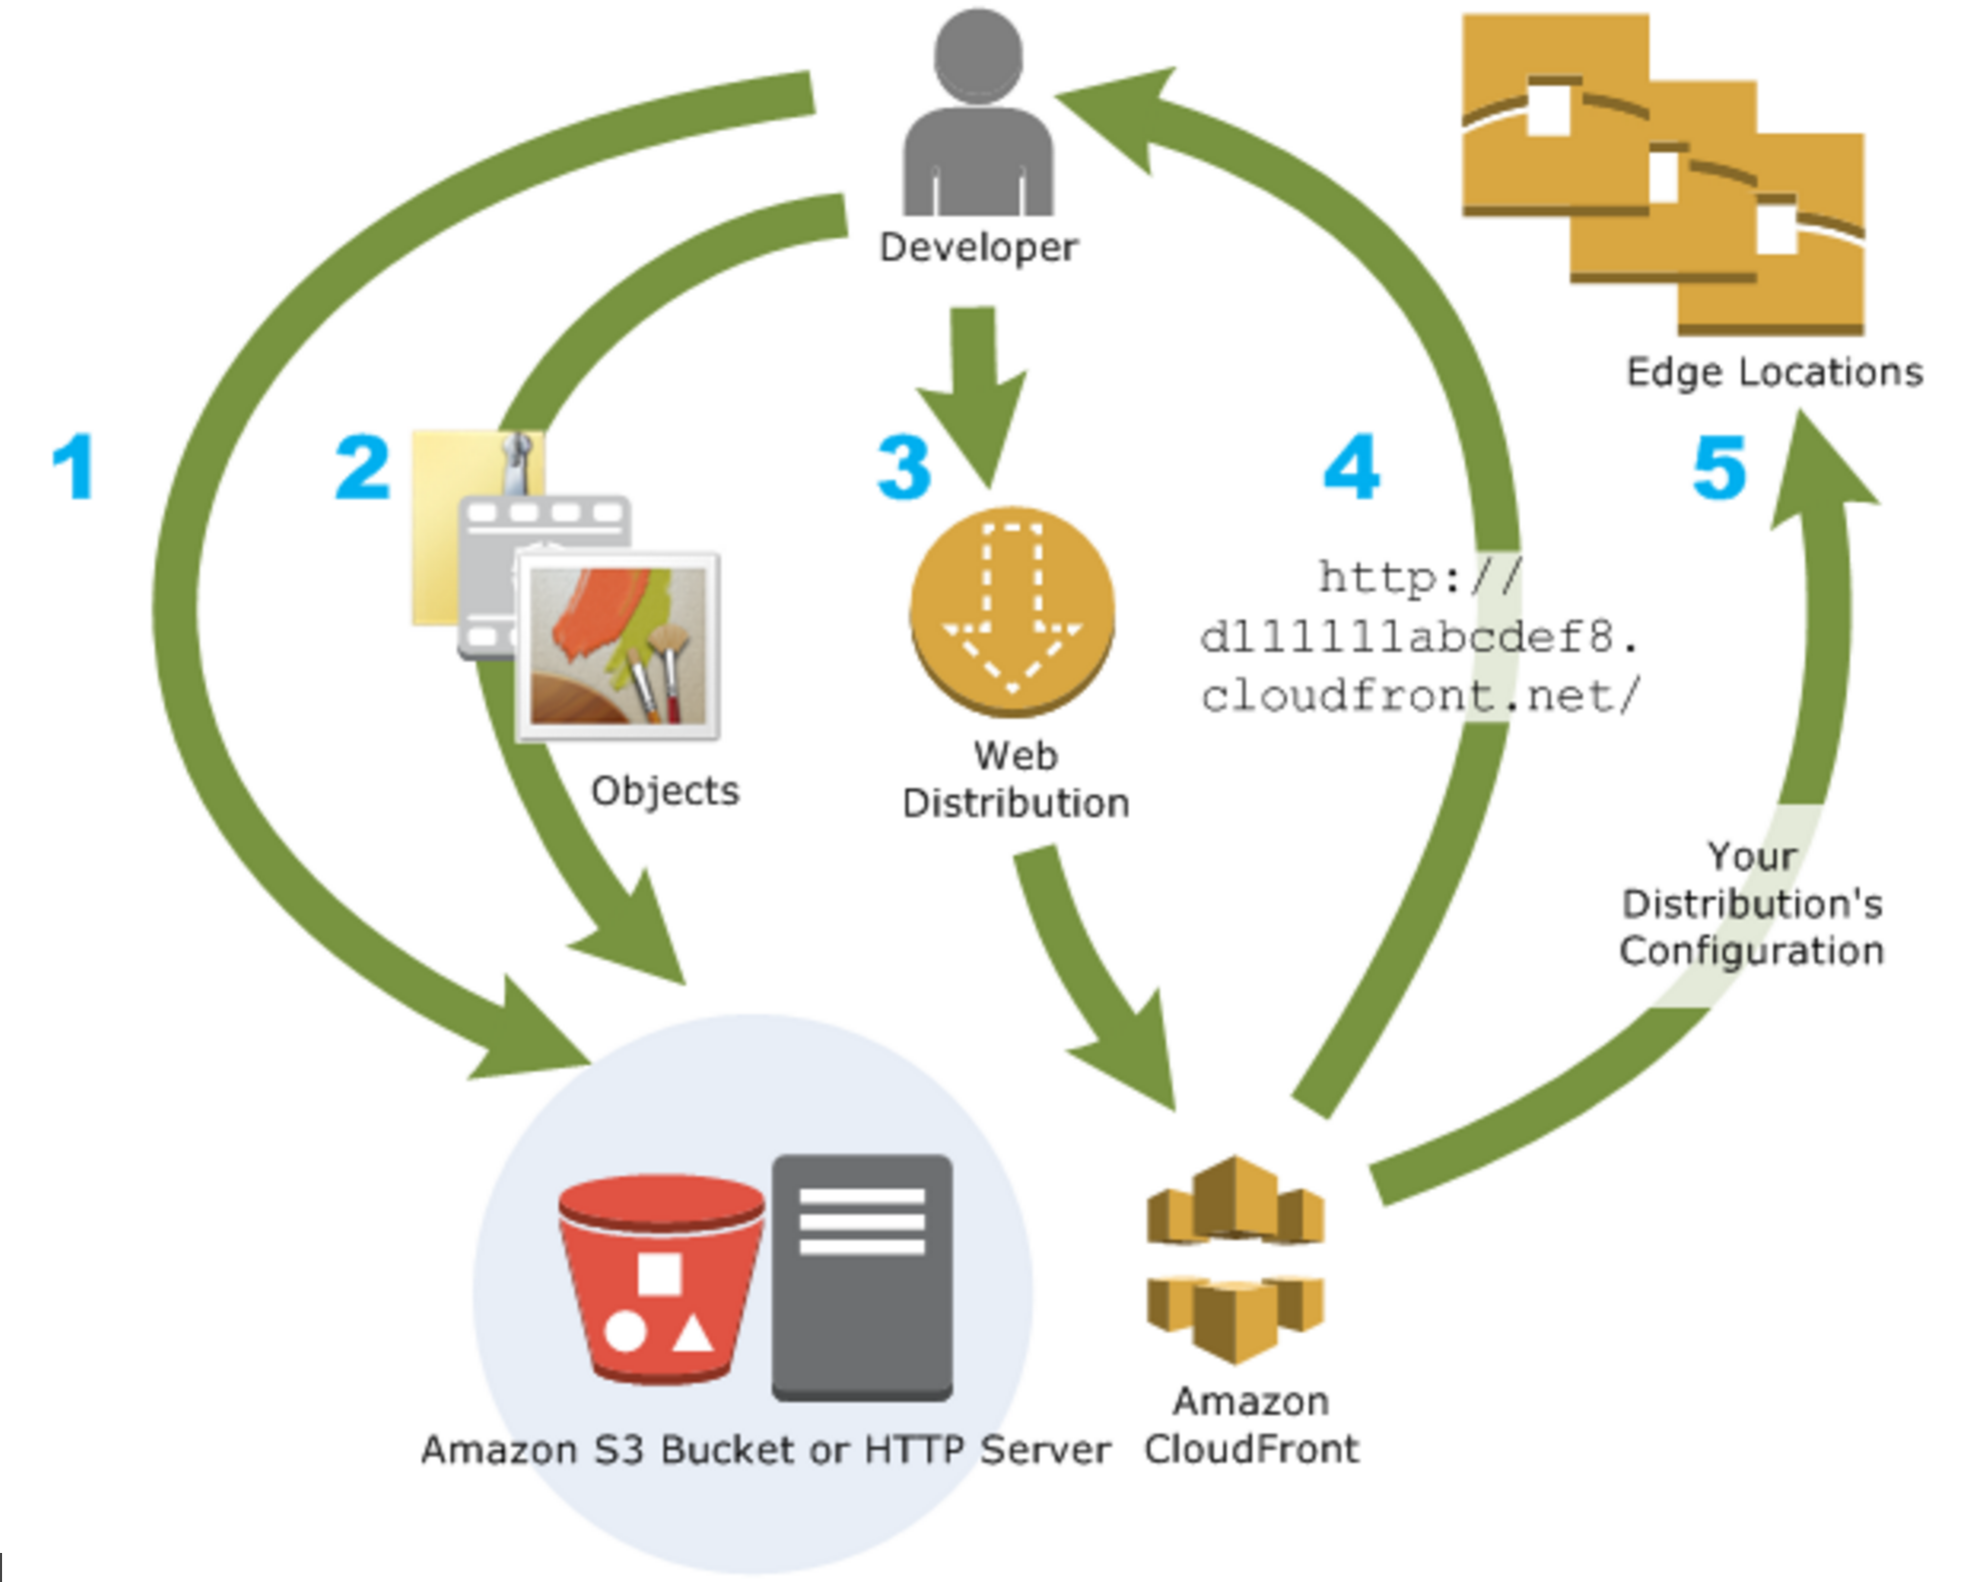
\includegraphics[width=1.0\linewidth]{images/chapter2/cloudfront.png}\hfill
 \caption[The CloudFront Lifecycle]{The CloudFront Lifecycle}
 \label{fig:fourV}
\end{figure}

When users request one or more objects DNS routes the request to the CloudFront edge location that can best serve the user's request, typically the nearest CloudFront edge location in terms of latency, and routes the request to that edge location.

In the edge location, CloudFront checks its cache for the requested files. If the files are in the cache, CloudFront returns them to the user. If the files are not in the cache, then forwards the request for the files to the applicable origin server for the corresponding file type.
CloudFront also adds the files to the cache in the edge location for the next time someone requests those files.
CloudFront forwards the next request for the object to your origin to determine whether the edge location has the latest version.
If the version in the edge location is the latest, CloudFront delivers it to your user.
If the version in the edge location is not the latest, your origin sends the latest version to CloudFront, and CloudFront delivers the object to your user and stores the latest version in the cache at that edge location.